\documentclass[11pt,oneside,a4paper]{memoir}
\usepackage{fontspec}
%\usepackage{showframe}
\usepackage{alltt}
\usepackage{xcolor}
\usepackage{tabu}
\usepackage{graphicx}
\usepackage{longtable}
\usepackage{multirow}
\usepackage{capt-of}
%\usepackage{wrapfig}
\usepackage[final]{listings}
\usepackage[unicode=true,xetex,colorlinks=true,linkcolor=blue,urlcolor=blue,bookmarksnumbered=true,bookmarksdepth=3]{hyperref}
\usepackage{bidi} % Must be last



%%%%%%%%%%%%%%%%%%%%%%%%%%%%%%%%%%%%%%%%%%%%%%%%%%%%%%%
%%%%%%%%%%%%%%%%%%%% Configuration %%%%%%%%%%%%%%%%%%%%
%%%%%%%%%%%%%%%%%%%%%%%%%%%%%%%%%%%%%%%%%%%%%%%%%%%%%%%

%%% Fonts %%%
\setmainfont[Ligatures=TeX]{Linux Libertine O}
\newfontfamily{\ezr}[Script=Hebrew]{EzraSIL}

\newfontfamily{\mainnolig}{Linux Libertine O}
\newcommand{\q}{{\mainnolig '}}


%%% Page layout %%%
\settypeblocksize{247mm}{160mm}{*}
\setlrmargins{*}{*}{1}
\setulmargins{*}{*}{1}
\checkandfixthelayout

%%% Hyperref (Information in PDF) %%%
\hypersetup{
unicode=true,
pdfauthor={Claus Tøndering},
pdftitle={Bible Online Learner: Users's Guide}
}

%%% Section numbering %%%
\setsecnumdepth{subparagraph}

%%% Lists %%%
\tightlists


%%% Colors %%%
\definecolor{dkgreen}{rgb}{0,0.6,0}
\definecolor{mauve}{rgb}{0.58,0,0.82}
\definecolor{shadecolor}{gray}{0.9}

%%% shaded environment %%%
\setlength{\FrameSep}{0.5\fboxsep}


%%% listings %%%
\lstset{frame=tb,
  aboveskip=3mm,
  belowskip=3mm,
  showstringspaces=false,
  keepspaces=true,
  columns=flexible,
  basicstyle={\footnotesize\ttfamily},
  numbers=none,
  numberstyle=\tiny\color{gray},
  keywordstyle=\color{blue},
  commentstyle=\color{dkgreen},
  stringstyle=\color{mauve},
  breaklines=true,
  breakatwhitespace=true,
  tabsize=3,
  escapechar=\%,
  captiondirection=LTR  % Required by bidi package (although its documentation says otherwise)
}

\renewcommand{\lstlistingname}{\textsc{Listing}}

\lstdefinelanguage{PHP}
{morekeywords={class,public,implements,function},
   morecomment=[l]//,
   morecomment=[s]{/*}{*/},
   morestring=[b]",
   morestring=[b]'
}

\lstdefinelanguage{TypeScript}
{morekeywords={class,interface,extends,string,number,boolean,any},
   morecomment=[l]//,
   morecomment=[s]{/*}{*/},
   morestring=[b]",
   morestring=[b]'
}

\lstdefinelanguage{CSS}
{
  moredelim={ [is][\color{blue}]{|}{|} },
  moredelim={ [is][\color{red}]{/}{/} }
}


%%% Chapter style %%%

% My own version of the ell chapter style:
\makechapterstyle{claus}{%
  \chapterstyle{default}
  \renewcommand*{\chapnumfont}{\normalfont\HUGE\sffamily}
  \renewcommand*{\chaptitlefont}{\normalfont\huge\sffamily}
  \settowidth{\chapindent}{\chapnumfont 111}
  \renewcommand*{\chapterheadstart}{\begingroup
    \vspace*{\beforechapskip}%
    \begin{adjustwidth}{}{-\chapindent}%
    \hrulefill
    \smash{\rule{0.4pt}{15mm}}
    \end{adjustwidth}\endgroup}
  \renewcommand*{\printchaptername}{}
  \renewcommand*{\chapternamenum}{}
  \renewcommand*{\printchapternum}{%
    \begin{adjustwidth}{}{-\chapindent}
    \hfill
    \raisebox{10mm}[0pt][0pt]{\chapnumfont\ifanappendix Appendix\else Chapter\fi\ \thechapter}%
                              \hspace*{1em}
    \end{adjustwidth}\vspace*{-3.0\onelineskip}}
  \renewcommand*{\printchaptertitle}[1]{%
    \vskip\onelineskip
    \raggedleft {\chaptitlefont ##1}\par\nobreak}}

% Default style should still use this font:
\renewcommand*{\chaptitlefont}{\normalfont\huge\sffamily}


%%% Indexing %%%

% Note: There is a problem with using \index in a (long)tabu* environment if the \index contains
% LaTeX commands, such as:
% \index{configuration JavaScript variable@\emph{configuration} JavaScript variable}
% Two things are required:
%    - The \emph must be preceded by \string
%    - The \index{...} must be replaced by \hmmindex{...} thus:
% \hmmindex{configuration JavaScript variable@\string\emph{configuration} JavaScript variable}}

\newcommand\hmmindex[1]{\index{#1}}

% Combines hyperref and italic page number in index
\newcommand*{\hyperit}[1]{\textit{\hyperpage{#1}}}

\renewcommand{\preindexhook}{Page numbers in italics are used to indicate the main references for an
  entry. A page number may appear both in italics and in upright letters if a term is used twice on
  a page.\label{sec-index}
\vspace{1cm}
}



%%% Auxiliary commands %%%
\newcommand*{\bibleref}[3]{#1~#2\thinspace:\thinspace#3}
\newcommand{\heb}[1]{{\RL {\ezr #1}}}
\newcommand{\forlater}[1]{} %Omit text
\newcommand*{\xml}[1]{\texttt{<#1>}}
\newcommand*{\xmla}[1]{\texttt{#1}} % An xml attribute


%%% Auxiliary tabu environments %%%
\tabulinesep=_2mm %Works together with the \addlinespace[...] values below

\newenvironment{my-longtabu}[2]{
%\begin{center}
\begin{longtabu*}{@{}#1@{}}
  \toprule
  #2\\\addlinespace[-1mm]
  \midrule
  \endhead

  \emph{\rmfamily\normalsize(Continued...)} & \\
  \endfoot

  \addlinespace[-1mm]\bottomrule
  \endlastfoot
}{%
\end{longtabu*}
%\end{center}%
}

\newcommand{\headii}[2]{\textbf{#1} & \textbf{#2}}
\newcommand{\headiii}[3]{\textbf{#1} & \textbf{#2} & \textbf{#3}}


% my-longtabu without \midrule
\newenvironment{my-longtabu-nomid}[2]{
\begin{center}
\begin{longtabu*}{@{}#1@{}}
  \toprule
  #2\\\addlinespace[-1mm]
  \midrule
  \endhead

  \emph{\rmfamily\normalsize(Continued...)} & \\
  & \\ % Required because the only instance of this table clashed with footnotes
  \endfoot

  \addlinespace[-1mm]\bottomrule
  \endlastfoot
}{%
\end{longtabu*}
\end{center}%
}

\newenvironment{my-tabu}[2]{%
\begin{center}
\begin{tabu}{@{}#1@{}}
  \toprule
  #2\\\addlinespace[-1mm]
  \midrule
}{%
\addlinespace[-1mm]\bottomrule
\end{tabu}
\end{center}%
}

%%% Allow extra space between words %%%
\sloppy

\captionnamefont{\small\itshape}
\captiontitlefont{\small\itshape}


\setfloatlocations{figure}{tb}

%% Command to select between to texts
\newcommand{\HOrG}[3]{\ifx#1h#2\else #3\fi}
\newcommand{\hebgr}{}   % Redefined in document
\newcommand{\hebgrlong}{}   % Redefined in document

%%% Front matter %%%
\title{Bible Online Learner:\\Technical Documentation}
\author{Claus Tøndering}
\date{16 May 2022}

\makeindex

\settocdepth{subsection}

\begin{document}
\begin{titlingpage*}
\maketitle

\begin{center}
Copyright © 2022 by Claus Tøndering, claus@tondering.dk

\vspace{5mm}

The document is made available under a Creative Commons Attribution 4.0 International License

(see \url{https://creativecommons.org/licenses/by/4.0/})
\end{center}
\end{titlingpage*}


\clearpage
\tableofcontents
\chapterstyle{claus} % TOC should be in default style. "claus" style starts here.

%%%%%%%%%%%%%%%%%%%%%%%%%%%%%%%%%%%%%%%%%%%%%%%%%%%%%%
%%%%%%%%%%%%%%%%%%%% Introduction %%%%%%%%%%%%%%%%%%%%
\chapter{Introduction}

\textbf{You should read this chapter.}
\plainbreak{3}

Bible Online Learner (or ``Bible OL'' for short) is a web-based computer program that supports
reading and learning biblical Hebrew and Greek. Bible Online Learner provides these features:


\begin{itemize}
\item Users can read the Old Testament in Hebrew and the New Testament in Greek.
\item Users can see grammatical information about the words and clauses in the text.
\item Teachers of Hebrew and Greek can create exercises based on the biblical texts.
\item Students can drill and test themselves using exercises created by teachers.
\item Teachers can keep track of how well students do in the exercises.
\item Teachers can generate exams for students.
\end{itemize}


%%%%%%%%%%%%%%%%%%%% How To Read This Document %%%%%%%%%%%%%%%%%%%%
\section{How To Read This Document}

This documents describes how to use Bible Online Learner (Bible OL). The document consists of three
parts:

\begin{itemize}
\item General information for everyone who wants to use Bible OL.
\item Information specifically for students who want to use the exercises provided in Bible OL.
\item Information specifically for teachers who want to create exercises in Bible OL.
\end{itemize}

At the start of most chapters you will find a line indicating if that chapter is relevant for you.

On page \pageref{sec-index} you will find an index, which may help you find your way through this document.

%%%%%%%%%%%%%%%%%%%%%%%%%%%%%%%%%%%%%%%%%%%%%%%%%%%%%%%%%%%%%
%%%%%%%%%%%%%%%%%%%% User Interface %%%%%%%%%%%%%%%%%%%%
\chapter{User Interface}

\textbf{You should read this chapter.}
\plainbreak{3}

You access Bible OL through a web browser using an appropriate
URL\footnote{Most users will use \url{https://bibleol.3bmoodle.dk}.}.

When you access the Bible OL main web site using a computer, you will see an introductory page,
at the top of which there is a menu. If you are using a smartphone, you will see a small rectangle with
three horizontal lines at the top right of the screen. Tap that rectangle to display the menu.


The menu has five items:

\begin{itemize}
\item \emph{Home} -- Selecting this item, takes you to the main web page.
\item \emph{Text and Exercises} -- This allows you to view the Hebrew and Greek biblical texts and to run exercises.
\item \emph{User Access} -- Here you can log in to the system and view the privacy policy.
\item \emph{Language} -- This lets you select the language of the user interface.
\item \emph{Variant} -- Here you can select between different variants of the terms and translations used. (See Section XXX.)
\end{itemize}


If you have a user account (see Section XXX), you can select Login from the User Access menu to
access your personal features of the system. Once you have logged, in, a new menu item appears:

\begin{itemize}
\item \emph{My Data} -- This menu item lets you change your user profile, setup font preferences, enroll in
  classes, and view how you are doing on the exercises.
\end{itemize}


%%%%%%%%%%%%%%%%%%%%%%%%%%%%%%%%%%%%%%%%%%%%%%%%%%%%%%
%%%%%%%%%%%%%%%%%%%% Viewing Text %%%%%%%%%%%%%%%%%%%%
\chapter{Viewing Text}\label{chap-viewing-text}

\textbf{You should read this chapter.}
\plainbreak{3}

The most basic operation of Bible OL is that of viewing the Hebrew or Greek text of the Bible.
From the \emph{Text and Exercises} menu select \emph{Display text.} This will take you to a web page
displaying the dialog of Figure \ref{fig-selecttext}.
\begin{figure}
  \begin{center}
    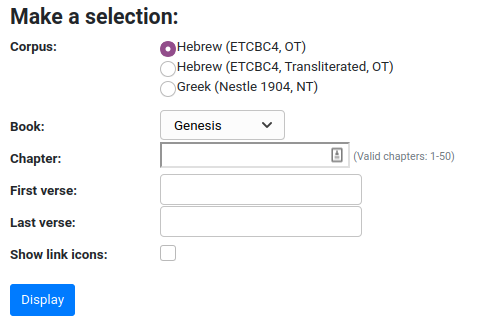
\includegraphics[width=0.6\textwidth]{selecttext.png}
  \end{center}
  \caption{Selecting a text to display.}\label{fig-selecttext}
\end{figure}
Under ``Corpus'' in that dialog, you select the text database you want to use. You have three options:


\begin{itemize}
\item \emph{Hebrew (ETCBC4, OT):} This is the Hebrew text of the Old Testament as provided by the ETCBC4
  database (see Appendix XXX).
\item \emph{Hebrew (ETCBC4, Transliterated, OT):} This is the Hebrew text of the Old Testament as provided by
  the ETCBC4 database, but written with Latin letters.
\item \emph{Greek (Nestle 1904,NT):} This is the Greek text of the New Testament as provided by the Nestle
  1904 database (see Appendix XXX).
\end{itemize}

Section \ref{sec-heb-view-text} shows how to use Bible Online Learner to study a Hebrew text.
Section \ref{sec-gr-view-text} shows how to study a Greek text. (You only need to read one of these
sections.)

\newcommand{\viewexampleI}[1]{%
%
\renewcommand{\hebgr}{\HOrG{#1}{heb}{gr}}
\renewcommand{\hebgrlong}{\HOrG{#1}{Hebrew}{Greek}}
%
\section{Viewing a \hebgrlong{} Text}\label{sec-\hebgr-view-text}

To see \HOrG{#1}{\bibleref{Genesis}{1}{1-7}}{\bibleref{Luke}{2}{1-5}}, fill out the dialog in figure \ref{fig-selecttext} thus:

\begin{itemize}
\item Corpus: \HOrG{#1}{Hebrew (ETCBC4, OT)}{Greek (Nestle 1904, NT)}
\item Book: \HOrG{#1}{Genesis}{Luke}
\item Chapter: \HOrG{#1}{1}{2}
\item First verse: 1
\item Last verse: \HOrG{#1}{7}{5}
\item Show link icons: Don’t mark this. (See Section XXX.)
\end{itemize}

Finally, click the \emph{Display} button. This will show you \HOrG{#1}{\bibleref{Genesis}{1}{1-7}}{\bibleref{Luke}{2}{1-5}} in \hebgrlong. (See Figure \ref{fig-\hebgr-text-a}.)
\begin{figure}
  \begin{center}
    \includegraphics[width=0.7\textwidth]{fig-\hebgr-text-a.png}
  \end{center}
  \caption{Displaying \HOrG{#1}{Genesis 1}{Luke 2}.}\label{fig-\hebgr-text-a}
\end{figure}

\HOrG{#1}{The small icon to the right of the first verse is a link to the same text at the SHEBANQ website.
(See Section XXX.)}


\subsection{Viewing \hebgrlong{} Grammar Information}\label{sec-\hebgr-grammar-info}

If you are viewing the text on a computer, you will have three ways to display grammar information;
if you are using a tablet or a smartphone, you will have two ways to display grammar information.
They are:

\begin{enumerate}
  \item Hovering the mouse over a word or sentence part. (This is not available on tablets or
    smartphones.)
  \item Clicking a word or sentence part.
  \item Using the ``MyView'' selector.
\end{enumerate}

On a computer, you can use your mouse to point to a word in the text.\footnote{Known as letting your
  mouse ``hover'' over a word.} You will then see a so-called \emph{grammar information
  box.}\index{grammar information box|hyperit}
to the right of the text as in Figure \ref{fig-\hebgr-text-b}.
\begin{figure}
  \begin{center}
    \includegraphics[width=\textwidth]{fig-\hebgr-text-b.png}
  \end{center}
  \caption{Displaying the grammar information box on a computer.}\label{fig-\hebgr-text-b}
\end{figure}
In this box you will see detailed information about the word your mouse points to. When you move the
mouse, the grammar information box disappears. You may find this inconvenient, so instead you can
use the following method:

On a computer, table, or smartphone, you can click or tap on a word. In that case, a dialog box will
appear containing the grammar information box. (You can click the × at the top of the dialog box or
the Close button at the bottom of the box to close the dialog. Alternatively, press the ``Esc'' key
on your keyboard.)

A third way to display grammar information is to use the ``MyView'' selector as described in the
following section.

%%%%%%%%%%%%%%%%%%%% The Grammar Selection Box %%%%%%%%%%%%%%%%%%%%
\subsection{The ``MyView'' Selector}\label{sec-\hebgr-myview-selector}\index{MyView@``MyView'' selector}

Above the \hebgrlong{} text you see an ``eye'' labelled ``MyView''. If you click the eye icon labelled
\emph{grammar selection box}\index{grammar selection box}. At the same time the eye icon turns into
a × icon. The grammar selection box looks as shown in Figure \ref{fig-\hebgr-gram-sel-a}.

\begin{figure}
  \begin{center}
    \includegraphics[width=0.7\textwidth]{fig-\hebgr-gram-sel-a.png}
  \end{center}
  \caption{\hebgrlong{} grammar selection box.}\label{fig-\hebgr-gram-sel-a}
\end{figure}

The \hebgrlong{} grammar selection box contains four buttons, identifying the four levels of the
grammar hierarchy used by the \hebgrlong{} text: The text contains \emph{sentences,} which contain
\emph{\HOrG{#1}{clauses}{level 2 clauses},} which contain \emph{\HOrG{#1}{phrases}{level 1
    clauses},} which contain \emph{words.} You can click on each of these to display relevant
grammar information.

If, for example, you click the \emph{Word} button and then the \emph{Lexeme} button, the grammar
selection box looks as shown in Figure \ref{fig-\hebgr-gram-sel-b}.
\begin{figure}
  \begin{center}
    \includegraphics[width=0.7\textwidth]{fig-\hebgr-gram-sel-b.png}
  \end{center}
  \caption{\hebgrlong{} grammar selection box after clicking \emph{Word} and \emph{Lexeme}.}\label{fig-\hebgr-gram-sel-b}
\end{figure}
If you now click the \emph{Part of speech} button, the Hebrew text changes to look as in Figure
\ref{fig-\hebgr-text-c}, where you can see the part of speech of each word of the text.
\begin{figure}
  \begin{center}
    \includegraphics[width=0.7\textwidth]{fig-\hebgr-text-c.png}
  \end{center}
  \caption{\HOrG{#1}{Genesis 1}{Luke 2} with part-of-speech information.}\label{fig-\hebgr-text-c}
\end{figure}
You can add additional information by clicking the relevant buttons in the grammar selection box.

You can use the \emph{Clear grammar} all the selected grammar information, and you can use the ×
icon to hide the grammar selection box.

The grammar selection box also allows you to see borders between \HOrG{#1}{phrases, clauses,}{clauses} or sentences,
as well as grammatical information about each of these. If, for example, you click
\emph{\HOrG{#1}{Clause}{Clause level 1}}, and then select
\emph{Show border}, you will see the borders of each clause.

By pointing your mouse to the word ``\HOrG{#1}{Clause}{Clause1}'' on the border of a particular
Clause (or, alternatively, clicking the word ``\HOrG{#1}{Clause}{Clause1}''), a grammar information box
for the particular clause will be shown. (See Figure \ref{fig-\hebgr-text-d}.)

\begin{figure}
  \begin{center}
    \includegraphics[width=\textwidth]{fig-\hebgr-text-d.png}
  \end{center}
  \caption{Showing grammar information for the second clause of \HOrG{#1}{Genesis 1}{Luke 2}.}\label{fig-\hebgr-text-d}
\end{figure}

\HOrG{#1}{Sometimes clauses (or other parts of a sentence) can contain other clauses inside them. An example
  of this is seen in \bibleref{Genesis}{1}{7} (Figure \ref{fig-\hebgr-text-e}). Here, you can see how the
  clause \heb{וַיַּבְדֵּ֗ל בֵּ֤ין הַמַּ֨יִם֙ וּבֵ֣ין הַמַּ֔יִם} is split in two and contains the clause \heb{אֲשֶׁר֙ מִתַּ֣חַת לָרָקִ֔יעַ} inside it.
  The split clause is marked by its missing left and right borders.

\begin{figure}
  \begin{center}
    \includegraphics[width=0.6\textwidth]{fig-\hebgr-text-e.png}
  \end{center}
  \caption{A split clause in \bibleref{Genesis}{1}{7}.}\label{fig-\hebgr-text-e}
\end{figure}
}{Some words may not belong to a particular clause, and a clause may be split into parts. In Figure
  \ref{fig-gr-text-d} the word καὶ at the start of verse 3 is not a member of a clause; and the
  clause in verse 1, the clause is split into two pars around the word δὲ, which is not part of the clause.
  The split clause is marked by its missing left and right borders.}

The different items you can select in the grammar selection box are detailed in section XXX, but
\HOrG{#1}{a few items are}{one item is} worth mentioning here:

In the grammar selection box, under \emph{Word} and \emph{Lexeme} you can enter a ``Word frequency
color limit''. Setting this value to, for example, 50, means that the 50 most common
\HOrG{#1}{Hebrew or Aramaic}{Greek} words in the \HOrG{#1}{Old}{New} Testament will be displayed in
black, whereas rarer words will be display in blue. (See Figure \ref{fig-\hebgr-text-f}.) If you are
learning \hebgrlong{}, you may find this feature useful when deciding if a word is worth memorizing.
When determining how common words are, different morphological forms of the same word are counted as
one. For more information about word frequency, see section XXX.

\begin{figure}
  \begin{center}
    \includegraphics[width=0.7\textwidth]{fig-\hebgr-text-f.png}
  \end{center}
  \caption{The 50 most common words are black, rarer words are blue.}\label{fig-\hebgr-text-f}
\end{figure}

\HOrG{#1}{In most cases, the information you find in the grammar information box will be the same as
  what is shown between the lines using the ``MyView'' selector; but for glosses this is not the
  case. For example, in the grammar information box of Figure \ref{fig-\hebgr-text-b} you can see
  that the lexeme \heb{היה} is translated into English as ``be, happen, become, occur''. But if you
  open the ``MyView'' selector and choose \emph{Word} and \emph{Glosses} and \emph{English}, only
  the first gloss, ``be'', will be shown between the lines of Hebrew text. }{} } \FloatBlock

\viewexampleI{h}

\FloatBlock

\viewexampleI{g}


%%%%%%%%%%%%%%%%%%%%%%%%%%%%%%%%%%%%%%%%%%%%%%%%%%%%
%%%%%%%%%%%%%%%%%%%% Logging In %%%%%%%%%%%%%%%%%%%%
\chapter{Logging In}

\textbf{You should read this chapter.}
\plainbreak{3}

You can use Bible OL to display biblical text and run some exercises without logging in to the
system. But if you want to customize the way text is displayed and if you want to take full
advantage of the system, you should have an account and log in when you use Bible OL.

%%%%%%%%%%%%%%%%%%%% Creating An Account %%%%%%%%%%%%%%%%%%%%
\section{Creating An Account}\index{account}\index{creating an account|see {account, creating}}

You can create an account yourself, or you can have your teacher create an account for you.

To create an account yourself, select \emph{Login} from the \emph{User Access} menu. This brings up
the login page, where you can select \emph{Create a new account}, or -- if allowed by your
installation -- you can use an existing Google or Facebook account to log in.


%%%%%%%%%%%%%%%%%%%% Advantages of Having An Account %%%%%%%%%%%%%%%%%%%%
\section{Advantages of Having An Account}

When you are logged in using an account, you get a number of extra possibilities:

\begin{itemize}
\item You can customize the fonts used for displaying text.
\item You can join classes set up by your teacher and access exercises that anonymous users cannot
  access.
\item When you take an exercise, your progress can be recorded and you and your teacher can monitor
  and grade your progress.
\end{itemize}

When you are logged in, an extra menu item appears on the Bible OL website: ``My Data''. This menu
has these items:

\begin{itemize}
\item \emph{Font preferences} -- Use this to change the fonts used to display Hebrew or Greek.
\item \emph{Profile} -- Here you can change your name, e-mail address, preferred interface language,
  and password. (If you are logged in via Google or Facebook, you can only change your preferred
  interface language.)
\item \emph{Enroll/unenroll in class} -- Use this to join or leave a class. Classes are described in
  detail in Chapter XXX.
\item \emph{My performance} -- See how you are doing solving the exercises.
\end{itemize}


To log out, select \emph{Logout} from the \emph{User Access} menu.


%%%%%%%%%%%%%%%%%%%% Special Account Privileges %%%%%%%%%%%%%%%%%%%%
\section{Special Account Privileges}\index{account!privileges}\index{privileges|see {account, privileges}}

A system administrator may assign special privileges to your account. The special privileges are:

\begin{itemize}
\item Facilitator
\item Translator
\item Sysadmin
\end{itemize}

The facilitator and translator privileges are independent of each other. A user may have either or
both sets of privileges.

A sysadmin has all the privileges of both facilitators and translators plus additional privileges.



\subsection{Facilitator}\index{facilitator}\index{teacher}

As a facilitator (or teacher) you have the following additional rights on the system:

\begin{itemize}
\item Add, modify, or delete user accounts (except for facilitator, translator, or sysadmin accounts).
\item Create and manage exercises.
\item Create and manage exams.
\item Create and manage classes.
\item Monitor how the students in your classes are doing in the exercises.
\item Assign or remove facilitator privileges to other accounts.
\end{itemize}

When you are logged in with facilitator privileges, additional items appears in the ``My Data'' menu:

\begin{itemize}
\item \emph{Students' performance} -- See how your students are doing solving the exercises.
\item \emph{Grade Quizzes} -- Grade students' quizzes.
\item \emph{Grade Exams} -- Grade students' quizzes.
\end{itemize}

Additionally, you will see a new menu item ``Administration'' with these items:

\begin{itemize}
\item \emph{Users} -- Manage user accounts.
\item \emph{Classes} -- Manage classes.
\item \emph{Manage exercises.}
\item \emph{Manage exams.}
\end{itemize}


\subsection{Translator}\index{translator}

As a translator you have the right to modify the translation of

\begin{itemize}
\item The user interface.
\item The names for Hebrew and Greek grammatical terms.
\item The Hebrew and Greek lexicons.
\item Add new languages to the set of available languages.
\end{itemize}

When you are logged in with translator privileges, you will see a new menu item ``Administration'' with these items:

\begin{itemize}
\item \emph{Translate interface} -- Translate the user interface.
\item \emph{Translate grammar items} -- Translate the names for Hebrew and Greek grammatical terms.
\item \emph{Translate lexicon} -- Translate the Hebrew and Greek lexicons.
\item \emph{Download lexicon} -- Download a translation of a Hebrew or Greek lexicon.
\item \emph{Available translations} -- View the available translations and add new languages.
\end{itemize}

\subsection{Sysadmin}\index{sysadmin}\index{administrator}\index{system administrator}

As a sysadmin (or system administrator) you have all the privileges of facilitators and translators
plus these additional rights:

\begin{itemize}
\item Add, modify, or delete user accounts (including facilitator, translator, or sysadmin accounts).
\item Manage gloss links (see Section XXX).
\item Change ownership of exercises.
\item Manage exercises created by other facilitators.
\item Manage exams created by other facilitators.
\item Manage classes created by other facilitators.
\end{itemize}

The ``Administration'' menu will have one additional item:

\begin{itemize}
\item \emph{Gloss links} -- See Section XXX.
\end{itemize}


%%%%%%%%%%%%%%%%%%%%%%%%%%%%%%%%%%%%%%%%%%%%%%%%%%%%%%%%%%%
%%%%%%%%%%%%%%%%%%%% Running Exercises %%%%%%%%%%%%%%%%%%%%
\chapter{Running Exercises}\index{running exercises}\index{exercises!running}

\textbf{Read this chapter if you want to run or create exercises.}
\plainbreak{3}

In this section we will look at how you run an exercise. We will go through a couple of examples
that you can try out on the system.

NOTE: You need not be logged in to try the code in this example, but you may see some warnings if
you are not logged in.

Exercises are located in folders in much the same way files on a computer are located in folders.
You can access the exercises by selecting \emph{Exercises} from the \emph{Text and exercises} menu.
You will then see a list of folders that are found within the top level folder (Figure \ref{fig-top-level}).
\begin{figure}
  \begin{center}
    
\includegraphics[width=0.4\textwidth]{toplevel.png}
  \end{center}
  \caption{The top level exercise folder.}\label{fig-top-level}
\end{figure}
The contents of some folders are available to all students, but you will see that some of the
folders here are marked ``Restricted''. These are folders that are only available to students that
are enrolled in certain classes. Students' access to folders is controlled by teachers as described
in section XXX.

Section \ref{sec-heb-exer} gives examples of how to run a Hewbrew exercise. Section
\ref{sec-gr-exer} gives examples of how to run a Greek exercise. (You only need to read one of these
sections.)


\newcommand{\exerciseexampleI}[1]{%
%
\renewcommand{\hebgr}{\HOrG{#1}{heb}{gr}}
\renewcommand{\hebgrlong}{\HOrG{#1}{Hebrew}{Greek}}
%

\FloatBlock

\section{\HOrG{#1}{Hebrew}{Greek} Exercises}\label{sec-\hebgr-exer}

\subsection{Example: First \HOrG{#1}{Hebrew}{Greek} Exercise}\label{sec-\hebgr-exer-i}

(For a corresponding \HOrG{#1}{Greek}{Hebrew} exercise, see Section \HOrG{#1}{\ref{sec-gr-exer-i}}{\ref{sec-heb-exer-i}}.)

Find the folder named ``\HOrG{#1}{ETCBC4}{Nestle~1904}'' and click on that. Within that folder, you
will find another folder called ``demo''. If you click on that, you will see a list of all the
exercises found within that folder (Figure \ref{fig-\hebgr-folder}).
\begin{figure}
  \begin{center}
    \includegraphics[width=0.9\textwidth]{\hebgr-folder.png}
  \end{center}
  \caption{The \HOrG{#1}{ETCBC4}{Nestle~1904}/demo exercise folder.}\label{fig-\hebgr-folder}
\end{figure}

We will now focus on the exercise called ``demo1''. The person who created this exercise
will have configured it with a set of Bible passages that should be used for this exercises. If you
click on one of the numbers 5, 10, or 25 under the heading ``Select number of questions using preset
passages'', you will start an exercise with 5, 10, or 25 questions take from the pre-configured
Bible passages. If instead you click on one of the numbers 5, 10, or 25 under the heading ``Select
number of questions and specify your own passages'', you will be allowed to specify the Bible
passages yourself.

Click on the number 5 under ``...preset passages'' and the exercise will start. The system will show
you a random sentence from the specified Bible passages, for example, the one you see in Figure
\ref{fig-\hebgr-exer-i}.
\begin{figure}
  \begin{center}
    \includegraphics[width=0.7\textwidth]{fig-\hebgr-exer-i.png}
  \end{center}
  \caption{The first sentence of a \hebgrlong{} exercise.}\label{fig-\hebgr-exer-i}
\end{figure}
At the top of the exercise you see a short description -- in this case ``Please indicate
  the gender and number of these nouns and pronouns.'' If you click the button labelled
``Locate''\index{locate}, you will learn that this sentence is found in
\HOrG{#1}{\bibleref{Genesis}{1}{6}}{\bibleref{Matthew}{8}{26}}. As described in Section
\ref{sec-\hebgr-grammar-info}, you can see more information about each word by pointing to it with
your mouse (if you are using an ordinary computer), by clicking on it, or by using the ``MyView''
selector.

  In this example, the system has highlighted three nouns or pronouns in purple. Your task is to identify the
grammatical gender and number of each of these words.

Below the text you see a green bar. This will show your progress through the five sentences of this
exercise. Below the bar is a box in which you should provide your answers. This answer box provides
some information about the noun: In this case it its the actual text and the English translation of
the word. These items are known as the ``Display features'' (see Figure \ref{fig-\hebgr-exer-ia}).
Below the display features is the information that you are expected to provide: In this case it is
the gender and number of the word. These items are known as the ``Request features''.

\begin{figure}
  \begin{center}
    \includegraphics[width=0.7\textwidth]{fig-\hebgr-exer-ia.png}
  \end{center}
  \caption{Display features and request features.}\label{fig-\hebgr-exer-ia}
\end{figure}

The first noun, \HOrG{#1}{\heb{רָקִ֖יעַ}}{ἀνέμοις}, is shown in the top line of the answer box, and you
must identify its gender by clicking either \HOrG{#1}{``Masculine'', ``Feminine'', or ``Other
  value'',\footnote{``Other value'' is not relevant in this exercise.}}{``N/A'',\footnote{That is,
    ``Not applicable''. This means that the word has no gender, which is the case for pronouns such
    as ``I'' and ``you''.} ``Masculine'', ``Feminine'', or ``Neuter''.} and its
number by clicking either \HOrG{#1}{``Singular'', ``Plural'', ``Dual'', or ``Other
  value''.}{``N/A'', ``Singular'', or ``Plural''.}

After making your choices, you may then check your answer by clicking ``Check answer''. Figure
\ref{fig-ans-\hebgr-i} shows you what a correct and a wrong answer looks like.
\begin{figure}
  \begin{center}
    \includegraphics[width=0.7\textwidth]{fig-ans-\hebgr-i.png}
  \end{center}
  \caption{A correct and a wrong answer to a \hebgrlong{} exercise.}\label{fig-ans-\hebgr-i}
\end{figure}
If you don't know the answer, clicking the ``Show answer'' button will display the correct answer.

In this sentence there are three nouns. We can move on to the next noun,
\HOrG{#1}{\heb{תֹ֣וךְ}}{θαλάσσῃ}, by clicking the \raisebox{-0.2\baselineskip}{
\includegraphics[height=11pt]{right-angle.png}} symbol at the right side of the answer box.
A \raisebox{-0.2\baselineskip}{
\includegraphics[height=11pt]{left-angle.png}} symbol will then appear at the left side of the answer box, allowing you to move back
to the previous word.

When the last word in the sentence, \HOrG{#1}{\heb{מָּ֑יִם}}{γαλήνη}, is shown (Figure \ref{fig-\hebgr-exer-ii}), three
buttons appear below the answer box.
\begin{figure}
  \begin{center}
    \includegraphics[width=0.7\textwidth]{fig-\hebgr-exer-ii.png}
  \end{center}
  \caption{Showing the last word of the exercise question.}\label{fig-\hebgr-exer-ii}
\end{figure}
Use the ``Next'' button to move to the next sentence. When there are no more sentences, or if you
want to terminate the exercise prematurely, you can click either ``GRADE task'' or ``SAVE outcome''.
Both of these terminate the exercise. If you are not logged in, no further action is taken,
regardless of which of the two buttons you press. But if you \emph{are} logged in, ``GRADE task''
causes the system to stores your result internally and indicates to the teacher that your result may
be used for grading your progress. ``SAVE outcome'' also stores your result internally, but
indicates that you do not want your result to be used for grading.

\FloatBlock

\subsection{Example: Second \HOrG{#1}{Hebrew}{Greek} Exercise}\label{sec-\hebgr-exer-ii}

(For a corresponding \HOrG{#1}{Greek}{Hebrew} exercise, see Section \HOrG{#1}{\ref{sec-gr-exer-ii}}{\ref{sec-heb-exer-ii}}.)

We will now look at the exercise called ``demo2'' in the
``\HOrG{#1}{ETCBC4/demo}{Nestle~1904/demo}'' folder. Click on the number 5 under ``...preset
passages'' for that exercise. The system will show you a random sentence from the specified Bible
passages, for example, the one you see in Figure \ref{fig-\hebgr-exer-iii}.

\begin{figure}
  \begin{center}
    \includegraphics[width=0.7\textwidth]{fig-\hebgr-exer-iii.png}
  \end{center}
  \caption{A sentence from the exercise ``\HOrG{#1}{ETCBC4/demo2}{Nestle 1904/demo2}''.}\label{fig-\hebgr-exer-iii}
\end{figure}


Here, we have a sentence from \HOrG{#1}{\bibleref{Genesis}{3}{14}}{\bibleref{Luke}{8}{17}}. You will
immediately notice an important difference from the previous example: Some of the words have been
replaced by a number in parentheses. The reason is that in this case Bible Online Learner asks the user to
provide a word that is actually part of the text; therefore the word must not be shown in the
window. The system has therefore replaced the interesting words with numbers.

In this example, the answer box contains five lines labelled \HOrG{#1}{``Item number'', ``Lexeme
  (with variant)'', ``Gender'', ``Number'', and ``State''}{``Item number'', ``Lexeme'', ``Tense'',
  ``Mood'', ``Voice'', ``Person'', and ``Number''}. The item number refers to the number in
parentheses in the sentence. \HOrG{#1}{In this case we have moved through the words to the third
  word.}{} The lexeme is the dictionary form of the word in question, and the \HOrG{#1}{number,
  gender, and state}{voice, mood, person, number, and tense} should help you create the word form
that is actually in the text.

Your task is to type the word form that is found in the text\HOrG{#1}{, but without the Hebrew
  cantillation marks (which you rarely need to know in detail).}{ in lower case without
  accents.\footnote{The label ``Normalized'' refers to a version of the text without punctuation and
    certain accents.}} Below the empty field
  for the text, you will see a few buttons labelled with \hebgrlong{} characters. You can use these
  buttons to spell the correct word form, which in this case is \HOrG{#1}{\heb{יְמֵי}}{εστιν}. The key
  marked \HOrG{#1}{$\rightarrow$}{$\leftarrow$} is a backspace key that deletes the last character
  you entered. The small characters in the upper \HOrG{#1}{right}{left} corner can be used to type
  the \hebgrlong{} character on you computer keyboard, if you prefer to do so rather than to click
  with your mouse. (More about this in Section XXX.)

When you have entered your answer, you can use the ``Check answer'' button to verify that your
answer is correct.
}

\exerciseexampleI{h}
\exerciseexampleI{g}

\FloatBlock


\section{Variations to Exercises}\index{variations to exercises}\index{exercises!variations}

The exercises presented in the previous sections illustrate how most exercises work. However, a
teacher can vary certain details about the way exercises look to the student. These details are
listed in the following sections.

\subsection{Fixed Exercises}\index{order of exercises}\index{exercises!fixed}\index{exercises!order}

Normally, the sentences for exercises are chosen at random from a set of Bible passages. This means
that every time you run an exercise, you may see new sentences.

However, an exercise may be constructed to display a fixed set of questions in a fixed order. If
that is the case, you will always see the same sentences every time you run the exercise.

Furthermore, the student can normally choose between seeing 5, 10, or 25 questions in an exercise;
but a teach may restrict this number so that only a fixed number of questions can be shown.

If either the order of questions or the number of questions is fixed, the students cannot themselves
choose the Bible passages for the exercise.

\subsection{Sentence Context}\index{sentence context}\index{context}

Normally, an exercise will show you one sentence at a time. However, an exercise may be constructed
to display a few sentences surrounding the sentence in question. For example, Figure
\ref{fig-context} shows one sentence in grey before and after the sentence that the exercise is
concerned with.

\begin{figure}
  \begin{center}
    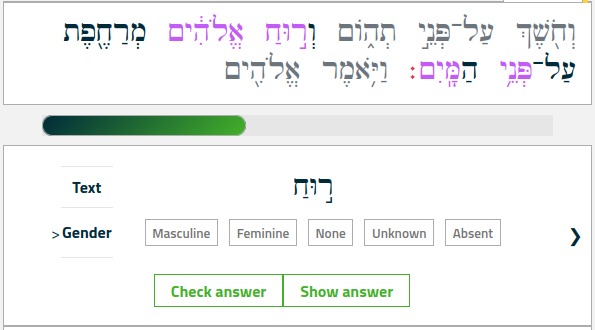
\includegraphics[width=0.7\textwidth]{fig-context.png}
  \end{center}
  \caption{Context around the sentence being considered is shown in grey. The sentence in question
    in shown in black and purple.}\label{fig-context}
\end{figure}


\subsection{Disabling ``Locate''}\index{disabling locate}\index{locate}

A teacher may disable the ``Locate'' button in an exercise.


\subsection{Hints}\index{hints}

Sometimes a Hebrew word form, taken on its own, may have multiple interpretations. For example, the
word form \heb{תֶחֱזֶה} can be both 2nd person masculine and 3rd person feminine. A teacher may
configure an exercise to provide hints to the correct interpretation. Figure \ref{fig-ambig} shows
a sentence where the student is asked to provide the gender for this particular word. A hint tells
the student that we are dealing with a 2nd person form, which aids the student in selecting the
correct gender, masculine.

\begin{figure}
  \begin{center}
    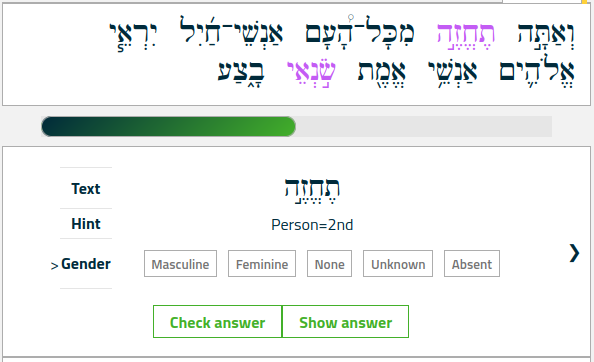
\includegraphics[width=0.7\textwidth]{fig-ambig.png}
  \end{center}
  \caption{An ambiguous word form with a hint.}\label{fig-ambig}
\end{figure}


\subsection{Hidden Information}

When viewing text outside an exercise, you have access to a considerable amount of grammatical
information. When doing an exercise, some of that information may be inaccessible, either because
the information would give away the correct answer, or because the teacher has deliberately hidden
some information.

As an example, consider the Hebrew exercise \emph{demo1} presented in section \ref{sec-heb-exer-i}, in
which you are required to provide the gender of a Hebrew noun. Gender information in normally
available via the ``MyView'' selector, but as Figure \ref{fig-no-gender} shows, the ``person,
gender, number'' button has been disabled. Also, hovering the mouse a word or clicking a word, will
not display gender information.

\begin{figure}
  \begin{center}
    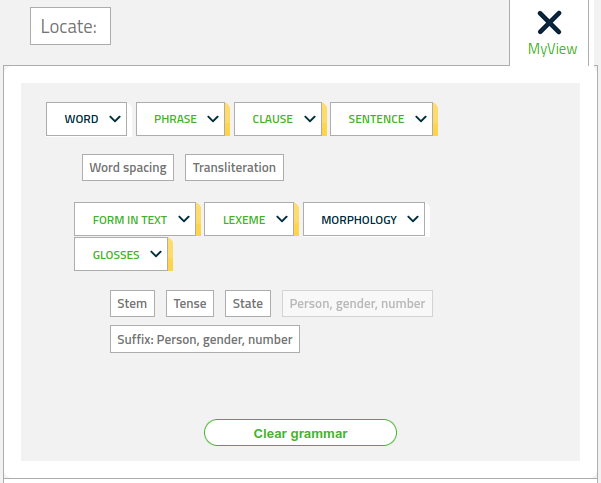
\includegraphics[width=0.7\textwidth]{fig-no-gender.png}
  \end{center}
  \caption{``Person, gender, number'' disabled.}\label{fig-no-gender}
\end{figure}



\begin{comment}
TODO:

Exercises about phrases and clauses.
Timeout warning

Tjek rækkefølge af display features i demo2. (Der kan være forskel på min og DBI's rækkefølge.)

Specialities: Typing nothing; entering glosses as answers; gloss limits.

Udskift billedet af filer i ETCBC4/demo or Nestle 1904/demo så man kan se øvelserne ``demo1'' og ``demo2''.

Nej, det er IKKE hvad ``Normalized'' betyder.

\end{comment}

%%%%%%%%%%%%%%%%%%%%%%%%%%%%%%%%%%%%%%%%%%%%%%%
%%%%%%%%%%%%%%%%%%%% Index %%%%%%%%%%%%%%%%%%%%
\printindex

\end{document}

% Local Variables:
% mode: latex
% ispell-dictionary: "british-ize"
% ispell-extra-args: ("--home-dir=/home/claus/Projects/BibleOL/usersguide")
% eval: (auto-fill-mode 1)
% End:
